\chapter[Probability Distribution Map and Task-Difficulty Map Editor Interface]{Probability Distribution Map and Task-Difficulty Map Editor Interface}
\label{chap:MapEdit}

At the \textbf{Between-Episodes} scale, a searcher might have additional case-specific information (e.g, past experience, knowledge of the search area or weather conditions, or the profile of the missing person) and would like to modify the general plan produced at the strategic scale. Moreover, as search progresses, the search plan should change due to newly found evidence (or the lack of it) from either the ground searchers or previous UAV flights. We developed two autonomy management tools at this scale that allow the user to manage two types of information: \textit{probability distribution map} and \textit{task-difficulty map}.

\begin{figure}
\centering
\begin{tabular}{cc}
	\begin{minipage}{0.45\textwidth}
	\centering
	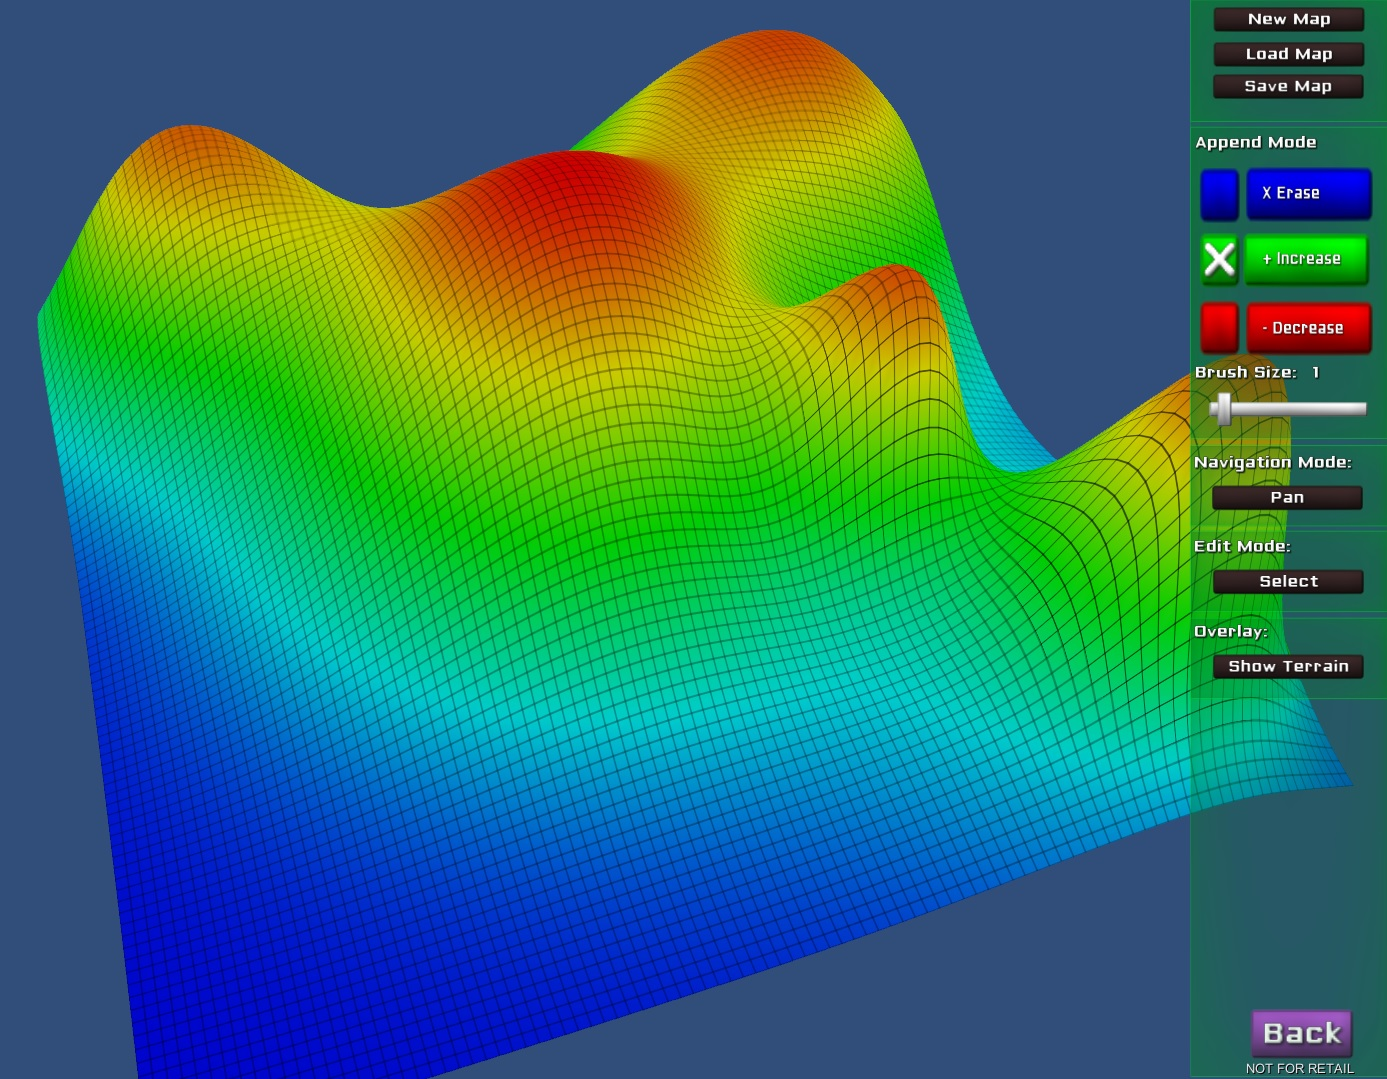
\includegraphics[width=2.8in]{DistEditExample.jpg}
	\caption{An example probability distribution map generated using the DistEdit tool.}
	\label{DistEditExample2}
	\end{minipage}
&
	\begin{minipage}{0.45\textwidth}
	\centering
	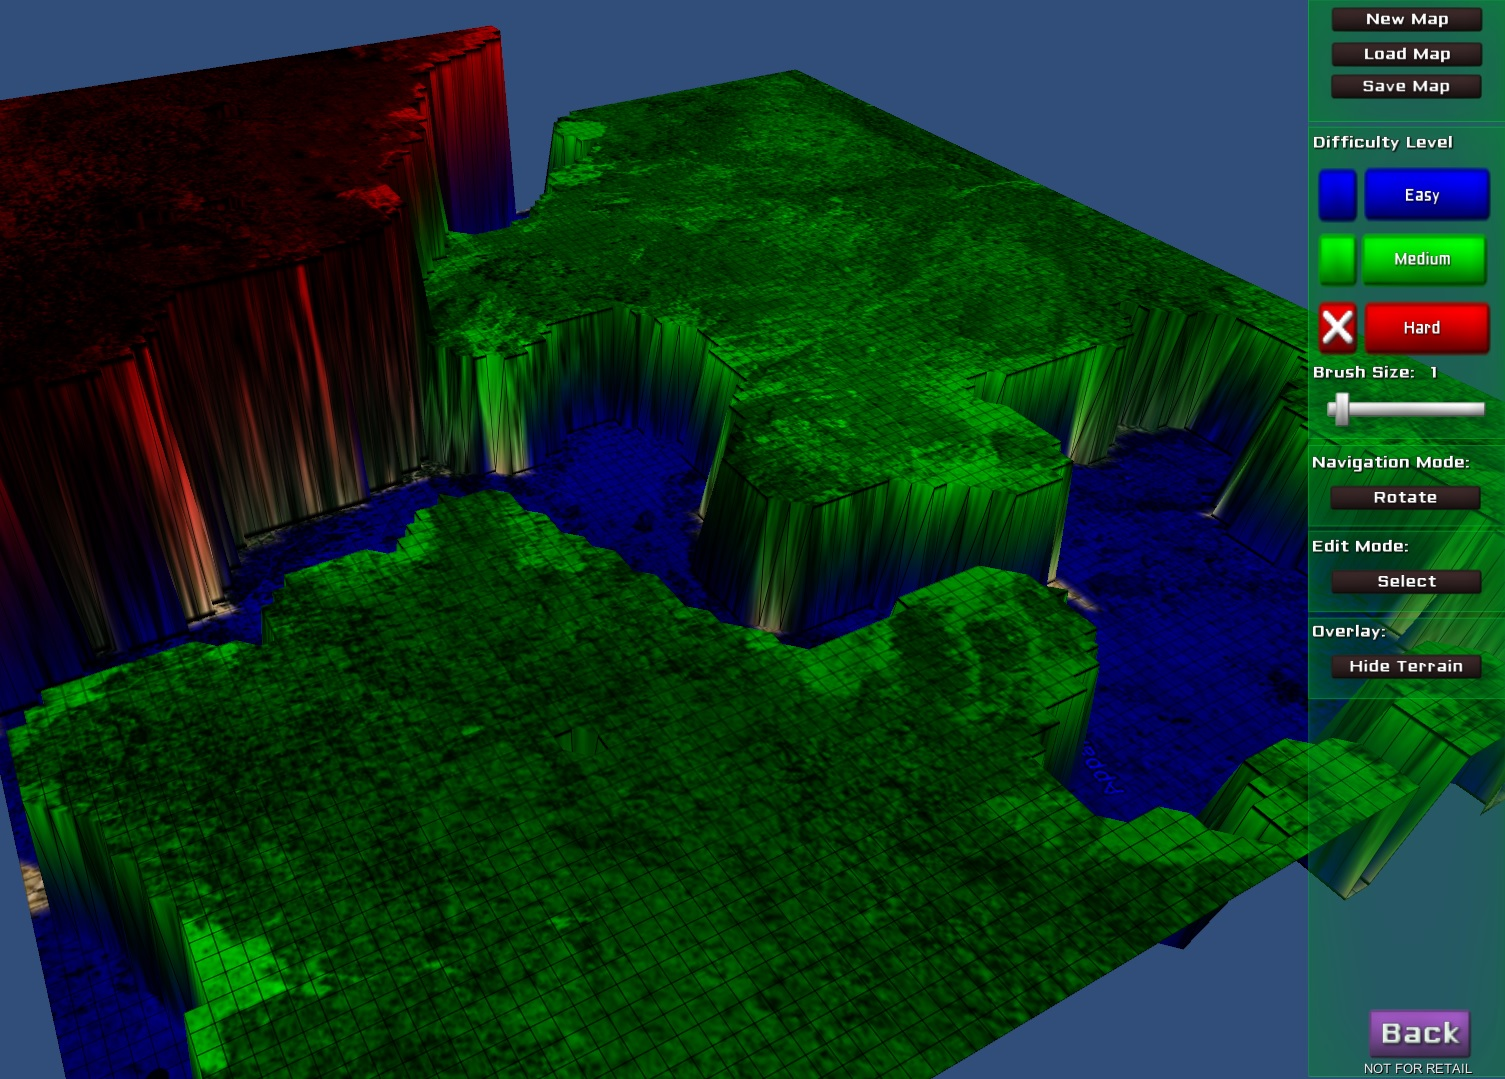
\includegraphics[width=2.8in]{DiffEditExample.jpg}
	\caption{An example task-difficulty map generated using the DiffEdit tool with satellite image of the search region overlaid on top.}
	\label{DiffEditExample2}
	\end{minipage}
\end{tabular}
\end{figure}

Searchers can use the \textbf{DistEdit} tool to modify a probability distribution map and use the \textbf{DiffEdit} tool to modify a task-difficulty map generated at the \textbf{Strategic} scale. Both tools enable the user to view maps as 3D surfaces where a color map is applied for better distinction (red means high probability area or high task-difficulty level and blue means low vise versa). The user can use mouse and finger gestures to rotate/pan/zoom the respective map and edit the shapes of the maps in 3D to incorporate information that the autonomous components are unable to interpret. The user also has the option to overlay a satellite image of the search area on top of the maps for better alignments.

if the user is dissatisfied with the \textit{probability distribution map} and \textit{task-difficulty map}.

%=====================================================================================================
\section{The DiffEdit Tool}
\label{}



In \textbf{DistEdit} the user can paint Gaussian distributions onto the probability distribution map (in the form of a 3D surface) with a paintbrush tool to specify \textit{areas of focus}. The mouse click (or finger press gesture) position determines the mean of the Gaussian distribution; brush size determines the standard deviation (with a radius equivalent to three times the standard deviation); and the duration of the click (or finger press gesture) determines the scale of the Gaussian distribution. Using this tool the user can add or subtract Gaussian components to the map to create a mixture of Gaussians. The modified probability distribution can be used later to prioritize tasks and plan UAV paths. By marking an area as a high priority area, the searchers can indirectly manipulate the UAV to search the area before other areas without the need to manually specify waypoints. Figure~\ref{DistEditExample2} shows an example probability distribution map generated using the \textbf{DistEdit} tool.

In \textbf{DiffEdit} the user can specify \textit{task difficulty} by using a paintbrush tool to paint on the task-difficulty map with scribbles. The user can also use a lasso tool to specify a region of irregular shape and then mark the region with selected task-difficulty level. By marking an area as a difficult area, the user can indirectly tell the UAV to make multiple passes over these areas to search more thoroughly. Figure~\ref{DiffEditExample2} shows an example task-difficulty map generated using the \textbf{DiffEdit} tool with the satellite image of the search region overlaid on top.

If the user does not like the probability distribution map or task-difficulty map generated at the \textbf{Strategic} scale, he or she can also use the \textbf{DistEdit} and \textbf{DiffEdit} tools to create new maps from scratch. Both tools enable the searchers to add additional information (especially the type of information autonomous components cannot interpret) to the intelligent system, relying on UAV path-planning to use the information to search more efficiently.




\begin{figure}
\centering
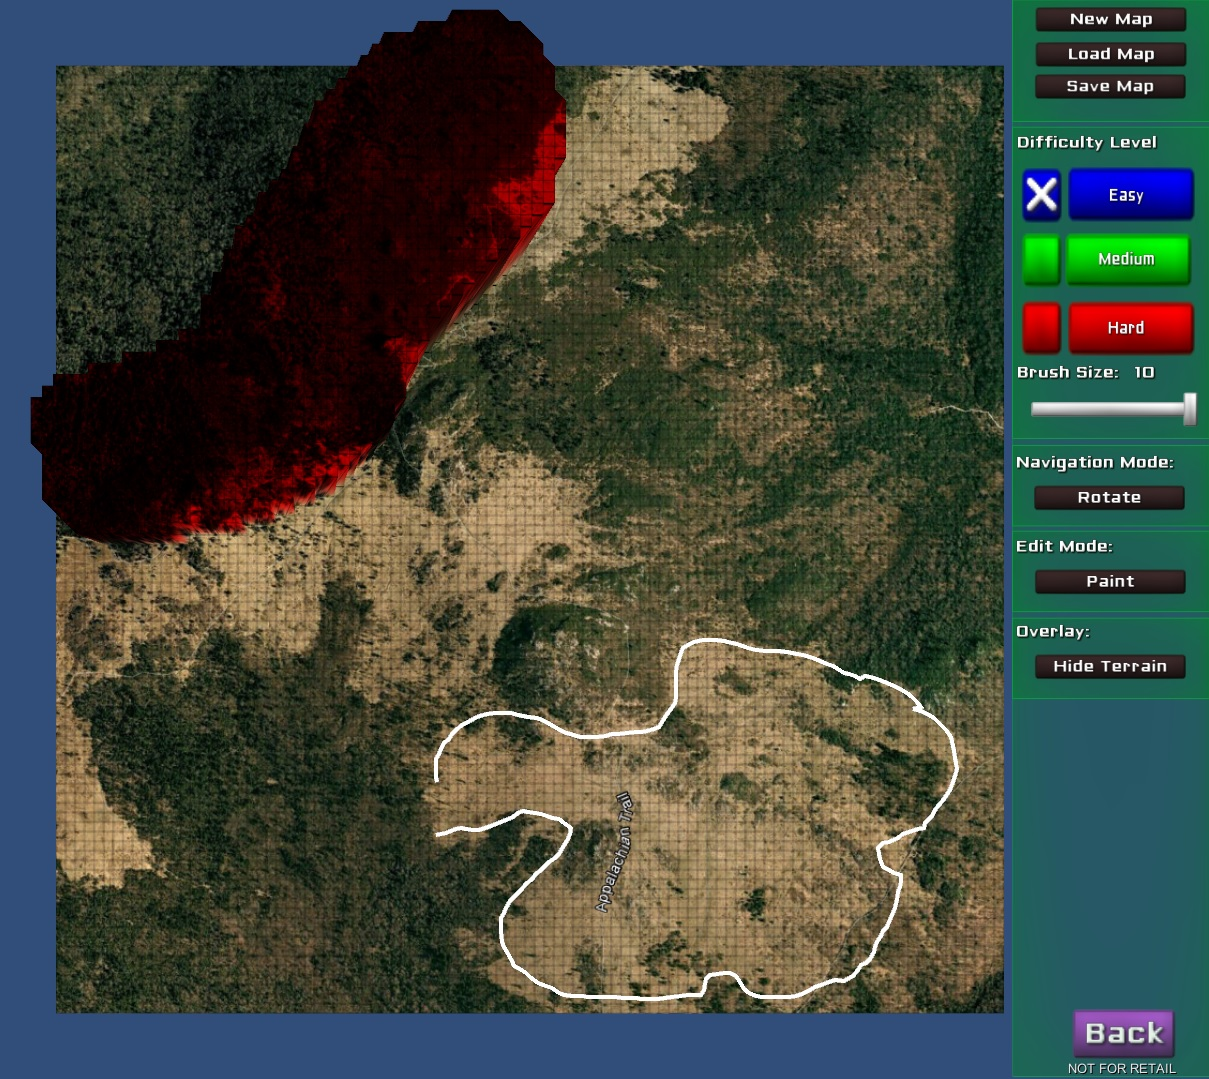
\includegraphics[width=6in]{DiffEdit001.JPG}
\caption{To be added}
\label{DiffEdit001}
\end{figure}

\begin{figure}
\centering
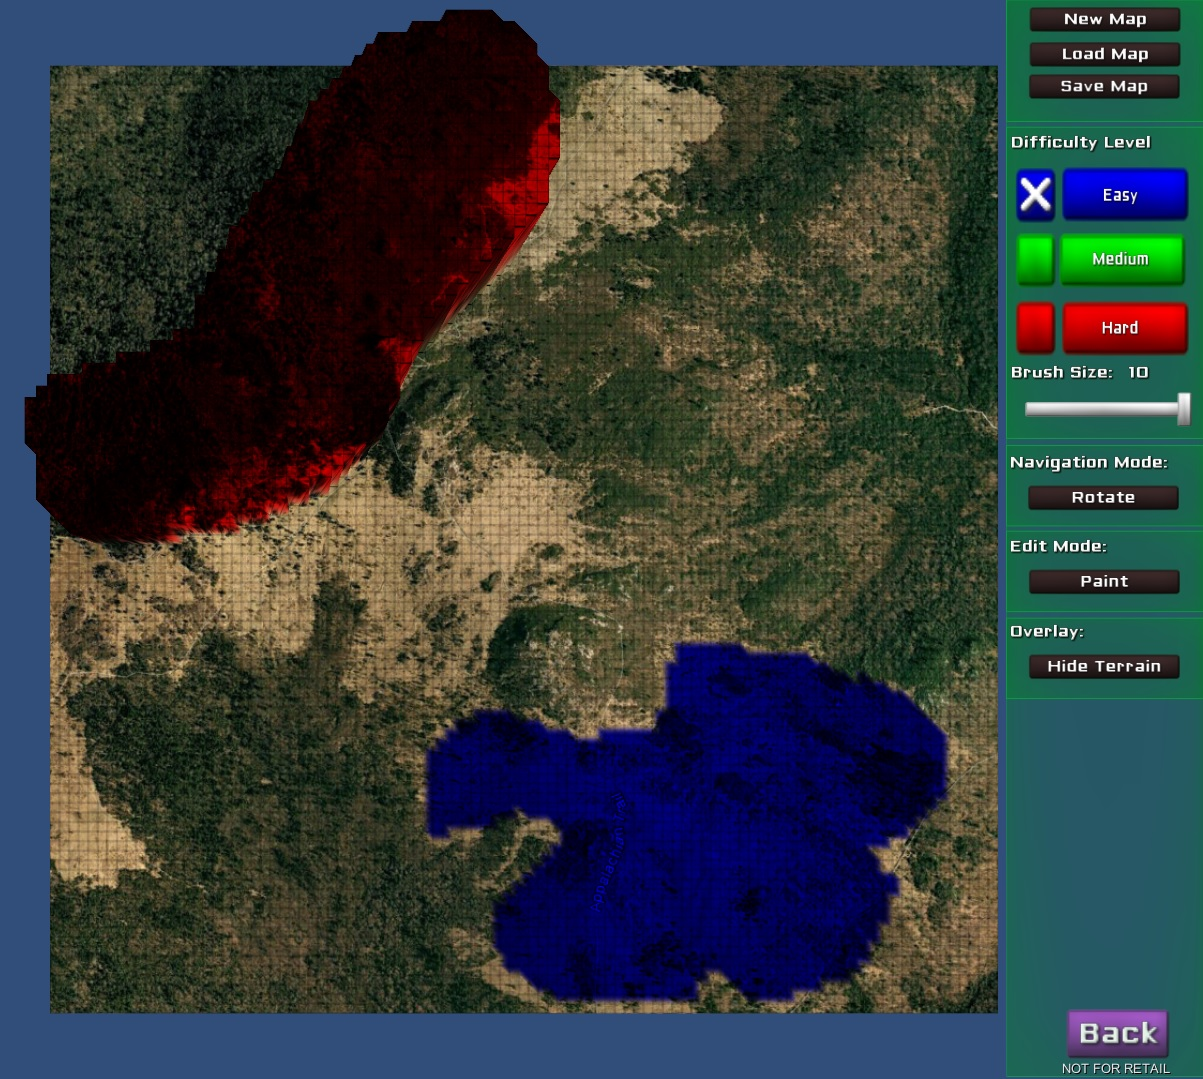
\includegraphics[width=6in]{DiffEdit002.JPG}
\caption{To be added}
\label{DiffEdit002}
\end{figure}

\begin{figure}
\centering
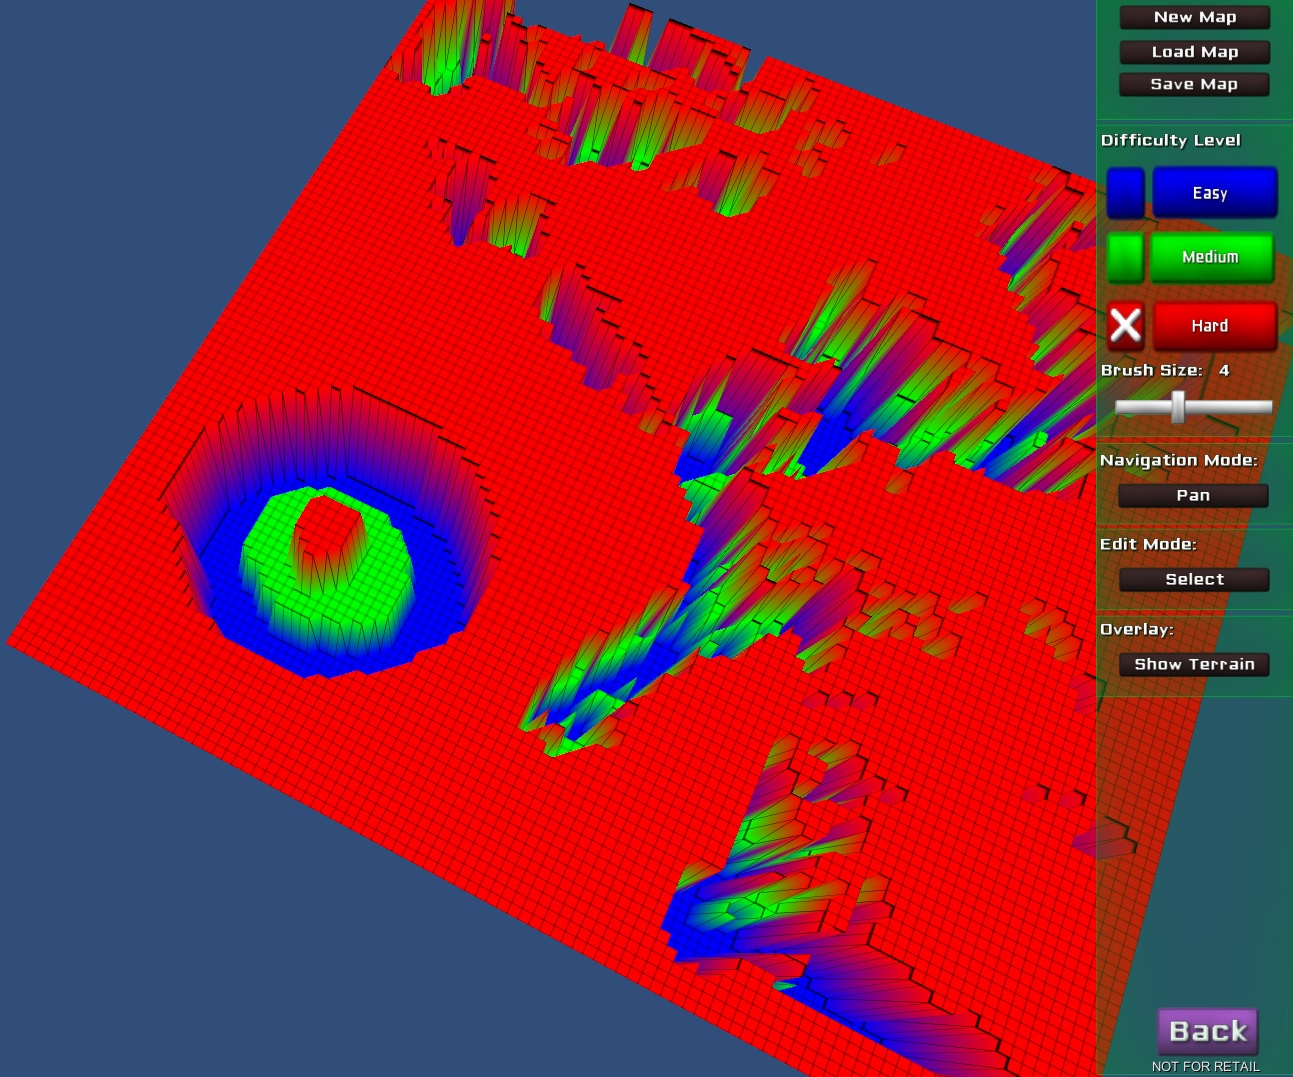
\includegraphics[width=6in]{DiffEdit003.JPG}
\caption{To be added}
\label{DiffEdit003}
\end{figure}


%=====================================================================================================
\section{The DistEdit Tool}


\begin{figure}
\centering
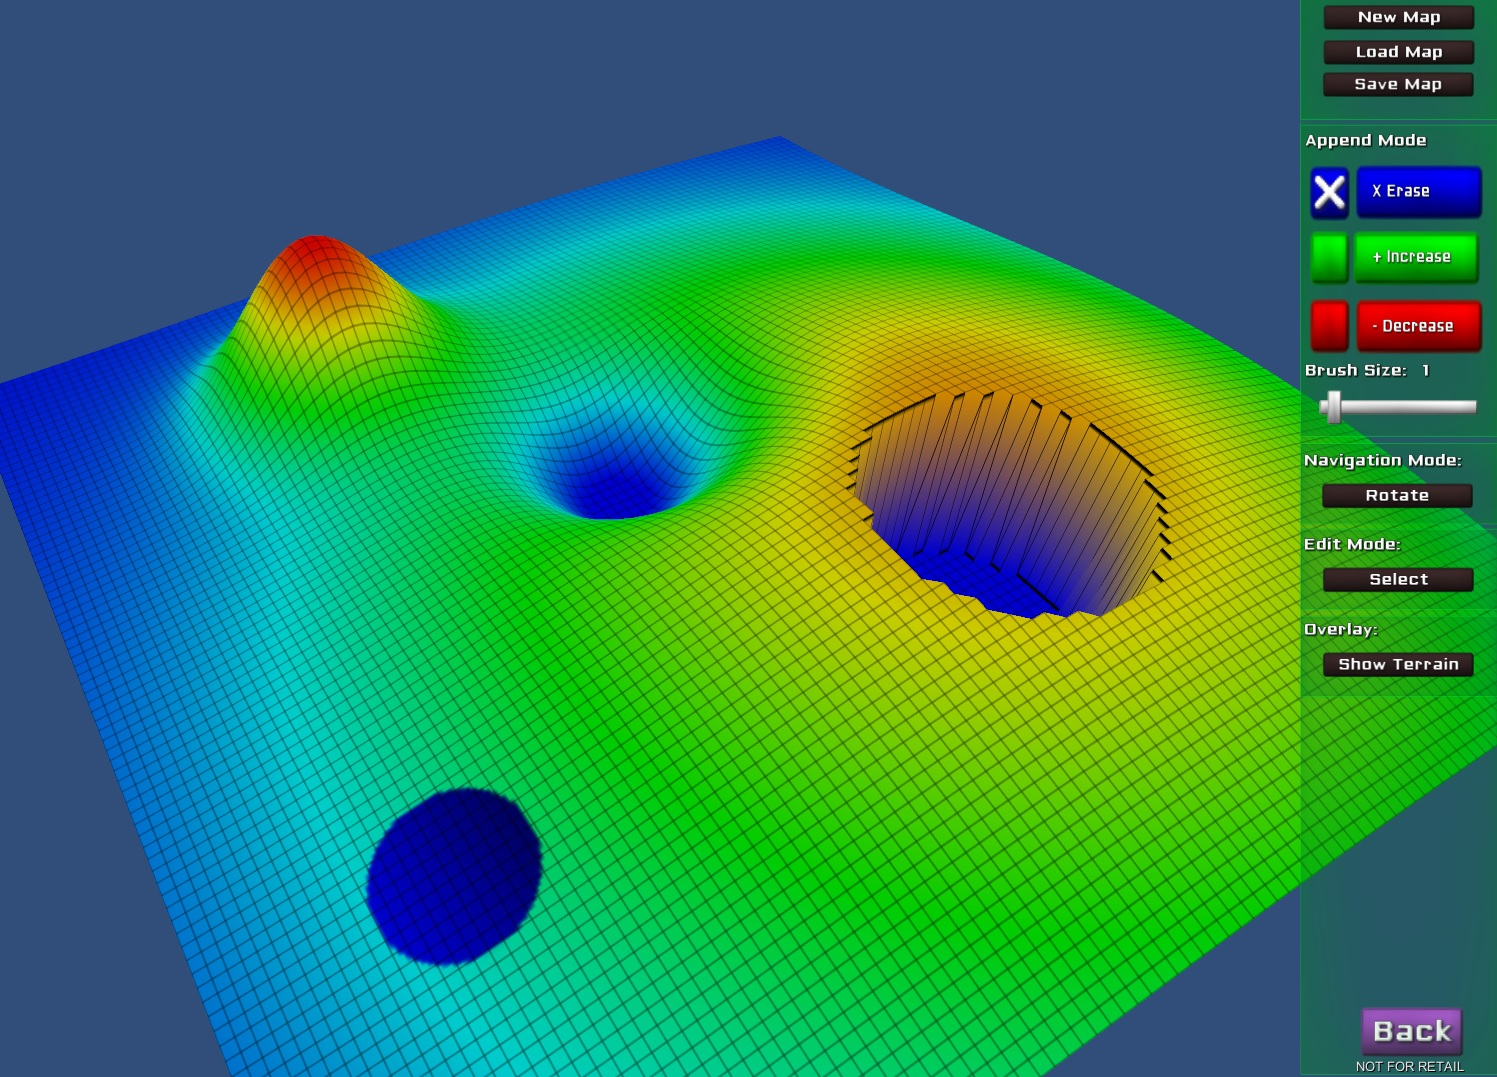
\includegraphics[width=6in]{DistEdit001.JPG}
\caption{To be added}
\label{DistEdit001}
\end{figure}

\begin{figure}
\centering
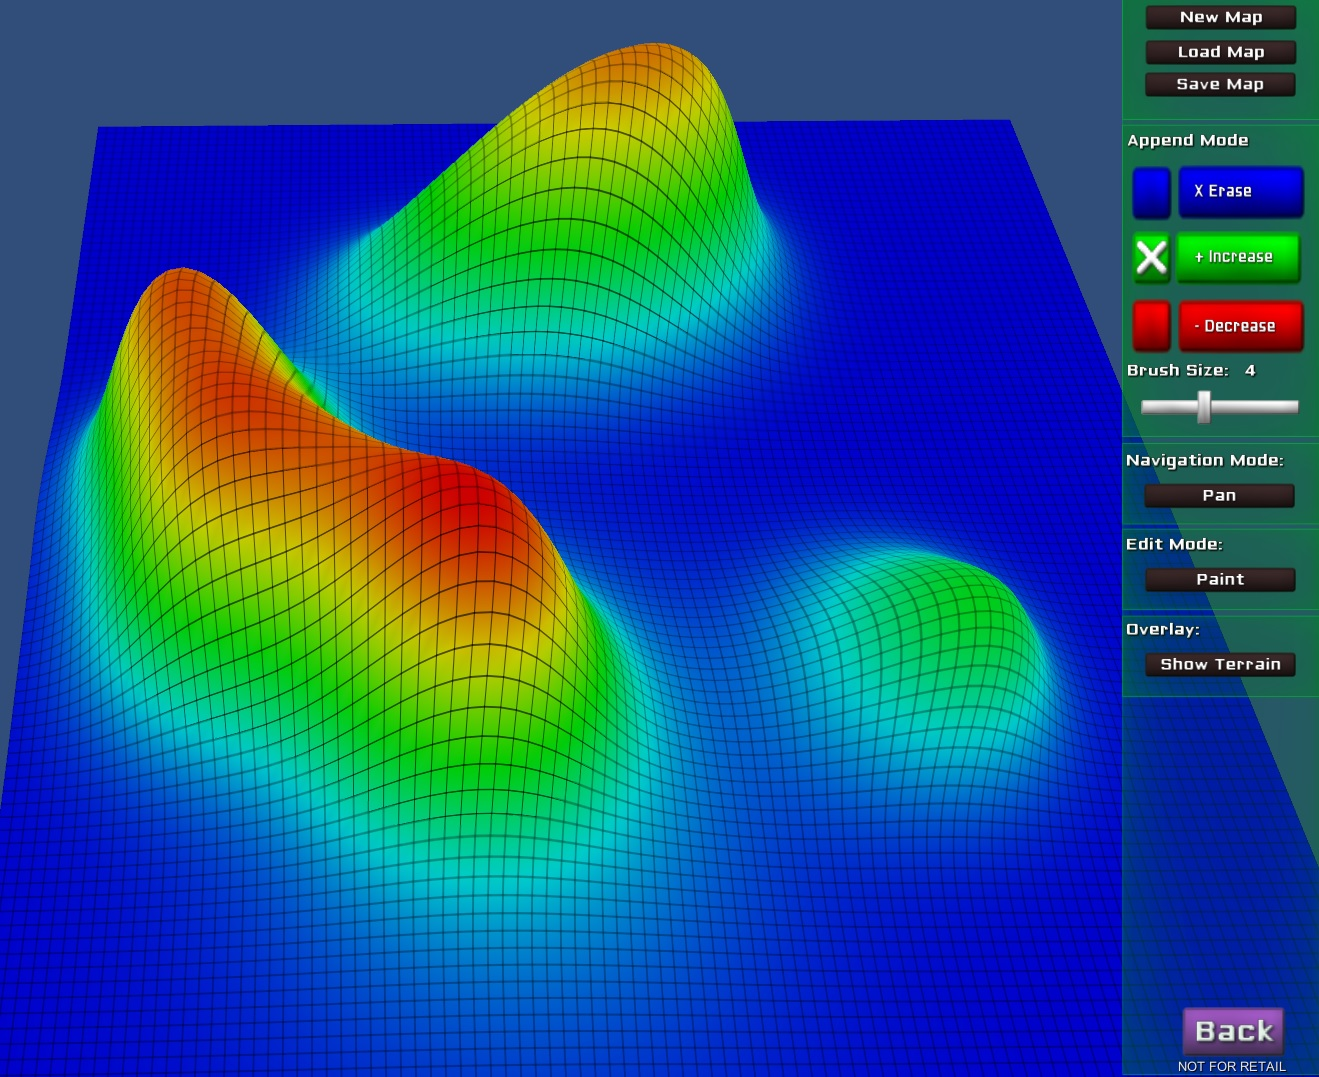
\includegraphics[width=6in]{DistEdit002.JPG}
\caption{To be added}
\label{DistEdit002}
\end{figure}

\begin{figure}
\centering
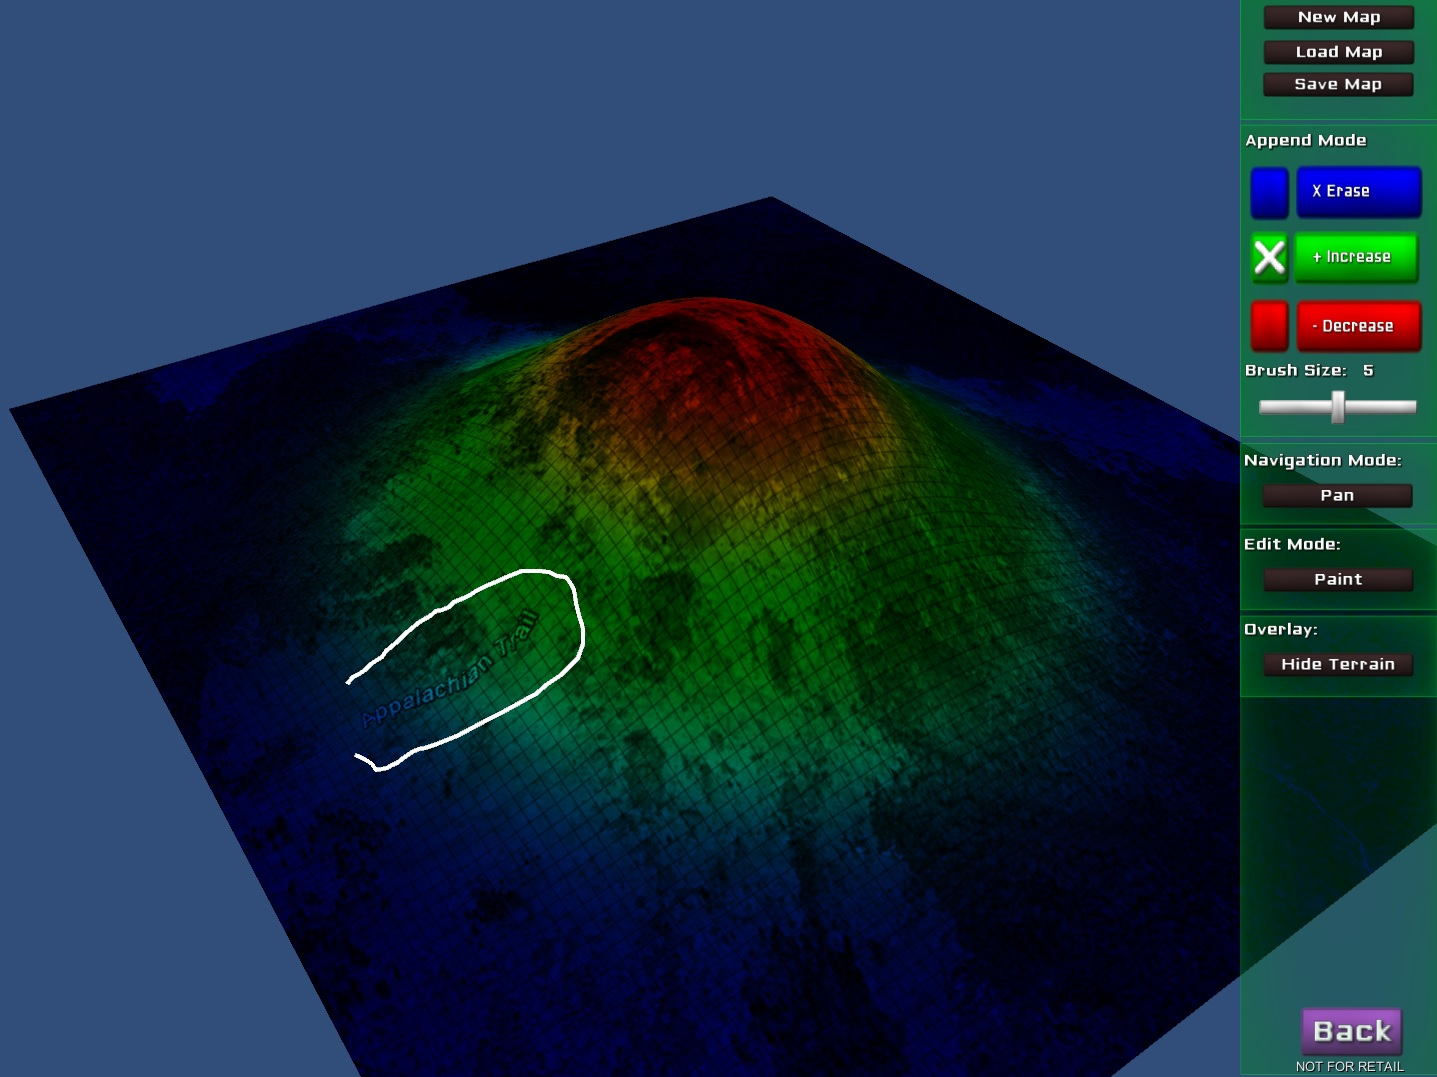
\includegraphics[width=6in]{DistEdit003.JPG}
\caption{To be added}
\label{DistEdit003}
\end{figure}

\begin{figure}
\centering
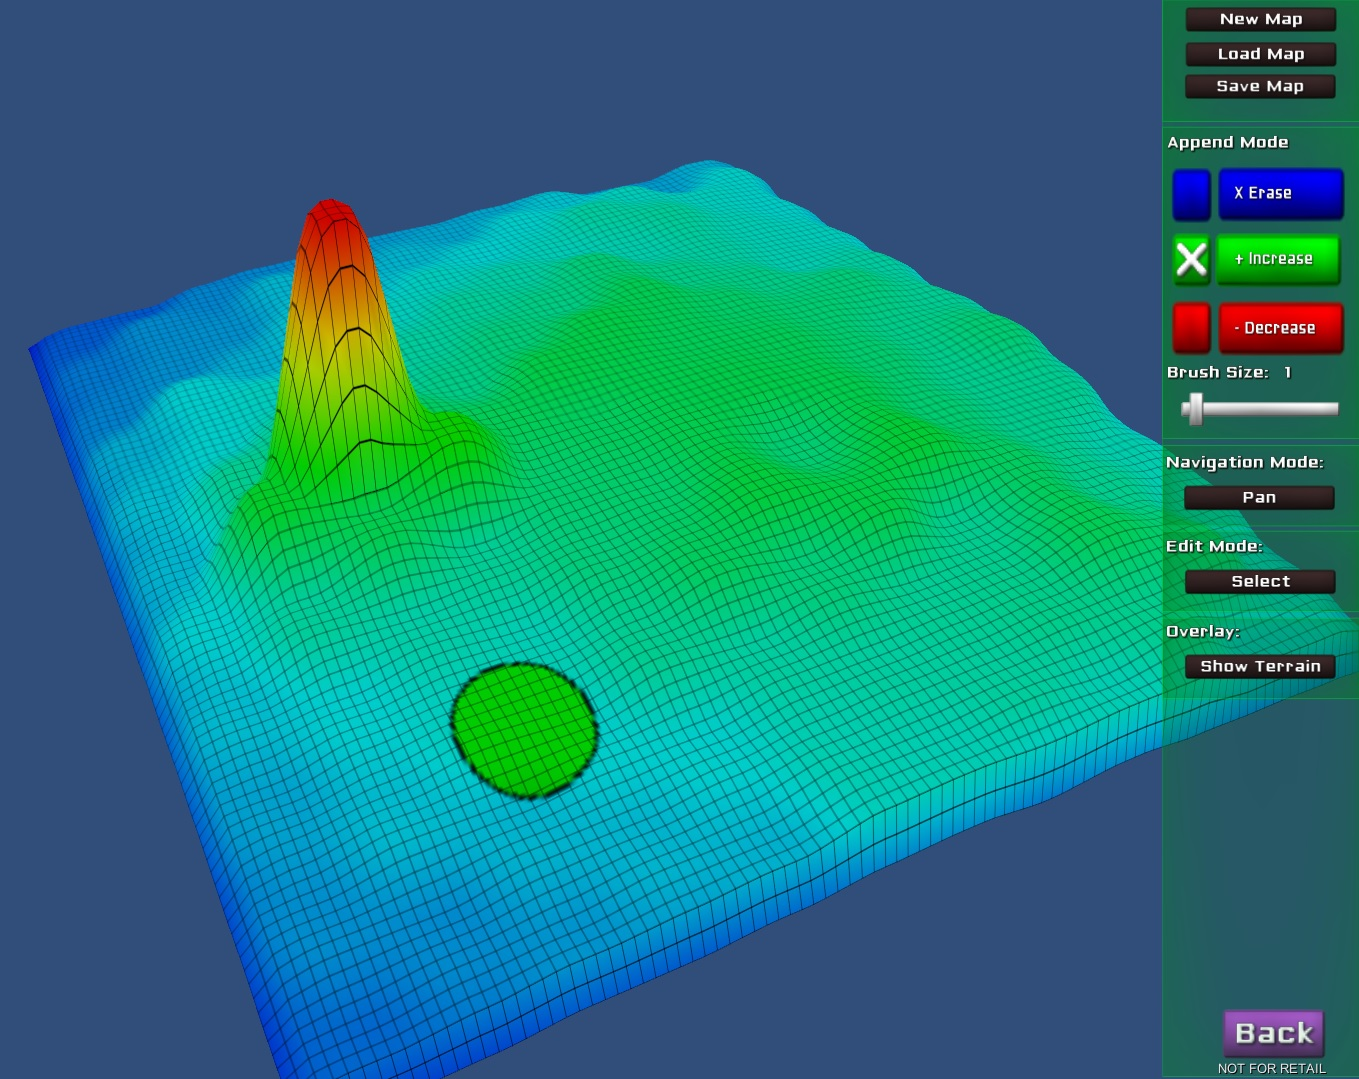
\includegraphics[width=6in]{DistEdit004.JPG}
\caption{To be added}
\label{DistEdit004}
\end{figure}

\begin{figure}
\centering
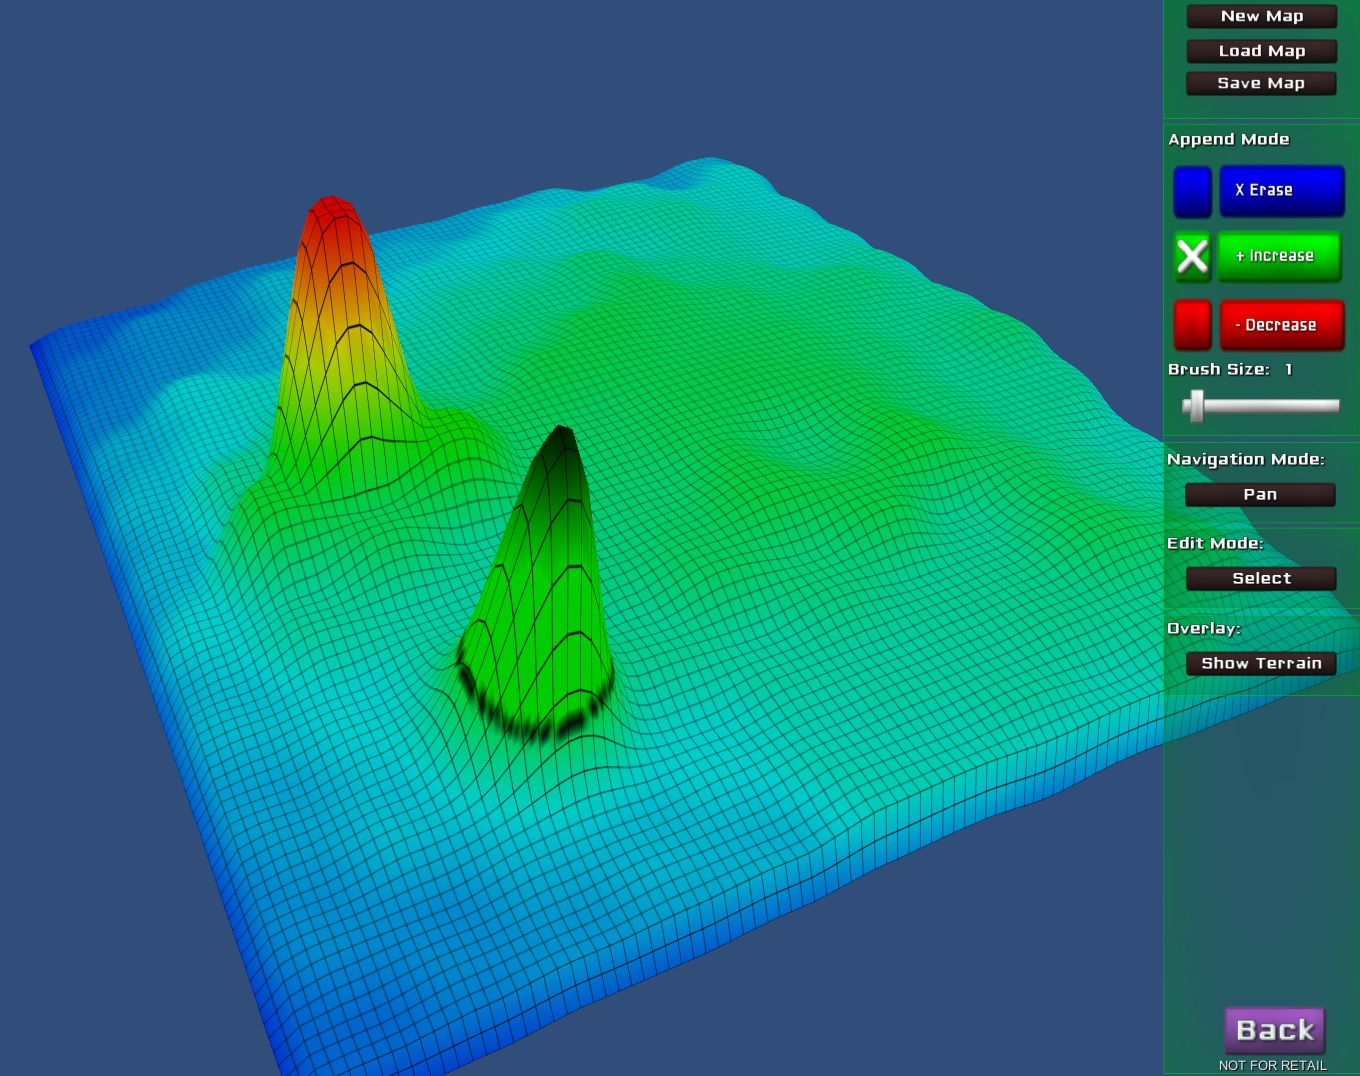
\includegraphics[width=6in]{DistEdit005.JPG}
\caption{To be added}
\label{DistEdit005}
\end{figure}


Searchers can use the \textbf{DistEdit} tool to modify a probability distribution map and use the \textbf{DiffEdit} tool to modify a task-difficulty map generated at the \textbf{Strategic} scale. Both tools enable the user to view maps in 3D with the option to overlay on top of the maps a satelite image of the search area. the user can using mouse gestures and finger gestures to rotate/pan/zoom the respective map and edit the shapes of the maps in 3D to incorporate information that the autonomous components are unable to interprete. 

The searchers can use simple mouse gestures (see Figure  for examples) to specify \textit{areas of focus} that will modify the probability distribution map (created at the strategic scale) using the proposed \textbf{DistMod} tool. Users will modify the distribution by making mouse gestures over a 2D representation of the distribution map where colors are used to represent the probability density (e.g., red for high probability hills and blue for low probability plains/valleys). The searchers can switch to a 3D view (read-only) for a better view of the distribution surface. The modified probability distribution can be used later to prioritize tasks and plan UAV paths. By marking an area as a high priority area, the searchers can indirectly manipulate the UAV to search the area before other areas without the need to manually specify waypoints. We will use the feature set developed by Dean Rubine~\cite{Rubine1991Specifying} and use the k-Nearest Neighbor algorithm~\cite{Mitchell1997Machine} for gesture recognition.

The proposed \textbf{DiffMod} tool allows the searchers to create or modify the \textit{task-difficulty map}. A searcher can pick a difficulty level from a color pallet and then either select a difficult area (maybe due to dense vegetations or low visibility) with lasso capability or paint the area using scribbles. By marking an area as a difficult area, the user can indirectly tell the UAV to make multiple passes over these areas to search more thoroughly.

Both tools enable the searchers to add additional information to the probability distribution and task-difficulty maps, relying on UAV path-planning to use the information to search more efficiently.

